\begin{surferPage}{Noch eine Cuspe ($A_2^{++}$ Singularität)}
Ganz ähnlich der vorigen Cuspen - Singularität ist diese hier; 
    die Gleichung hat sich im Verhältnis zur vorigen nur durch ein Vorzeichen
    verändert: 
    \vspace*{-0.4em}
    \begin{center}
      $x^3+y^2+z^2=0.$
    \end{center}
    \vspace*{-0.4em} Dies bewirkt, dass die Fläche nun rotations-symmetrisch
    ist, genauso wie ihre Deformation mit der Gleichung 
    $(1-a)x^3-ax^2+y^2+z^2=0$, $a>0$ in eine
    Singularität vom Typ $A_1^{+-}$: 
    \begin{center}
      \vspace*{-0.7em}
      \begin{tabular}{@{}c@{\quad}c@{\quad}c@{}}
        \begin{tabular}{@{}c@{}}
          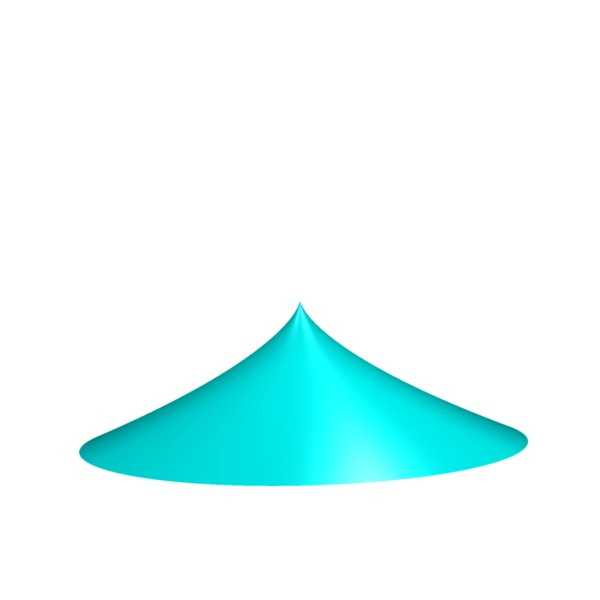
\includegraphics[width=1.2cm]{../../common/images/A2pp_0}
        \end{tabular}
        &
        \begin{tabular}{@{}c@{}}
          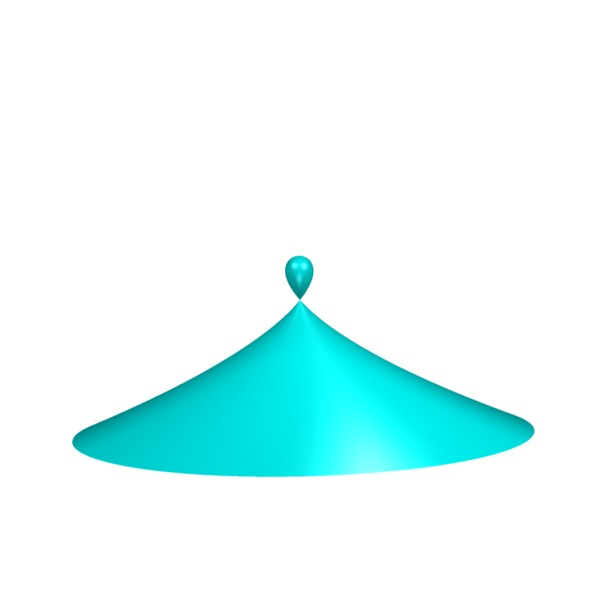
\includegraphics[width=1.2cm]{../../common/images/A2pp_1}
        \end{tabular}
        &
        \begin{tabular}{@{}c@{}}
          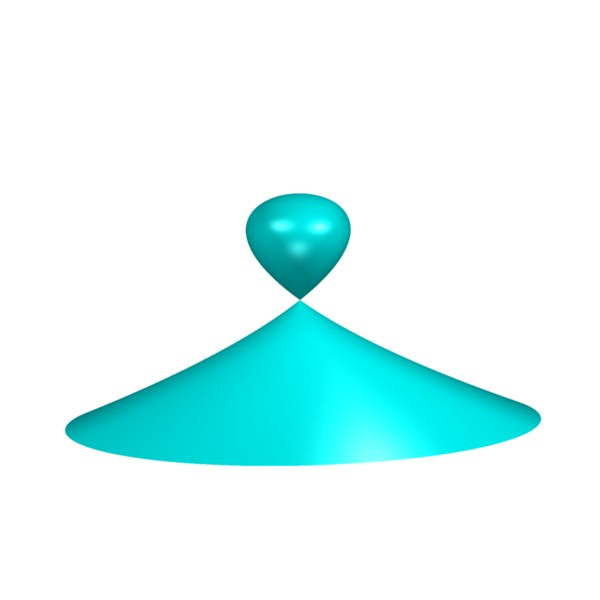
\includegraphics[width=1.2cm]{../../common/images/A2pp_2}
        \end{tabular}
      \end{tabular}
    \end{center}
    \vspace*{-0.4em}
    Die Rotations-Symmetrie in der $yz$- Ebene kann hier sehr einfach sehen:
    Schreibt man die Gleichung nämlich um in $y^2+z^2=-(x^3)$, so
    erkennt man, dass sich für jedes feste $x<0$ ein Kreis ergibt, da ja die
    Gleichung $y^2+z^2=r^2$ einen Kreis beschreibt. 

    Als Schnitte der deformierten Cuspe mit einer Ebene ergeben sich eine
    ebene Kuspe und eine ebene Schlaufe: 
    \begin{center}
      \vspace*{-0.7em}
      \begin{tabular}{@{}c@{\quad}c@{\quad}c@{}}
        \begin{tabular}{@{}c@{}}
          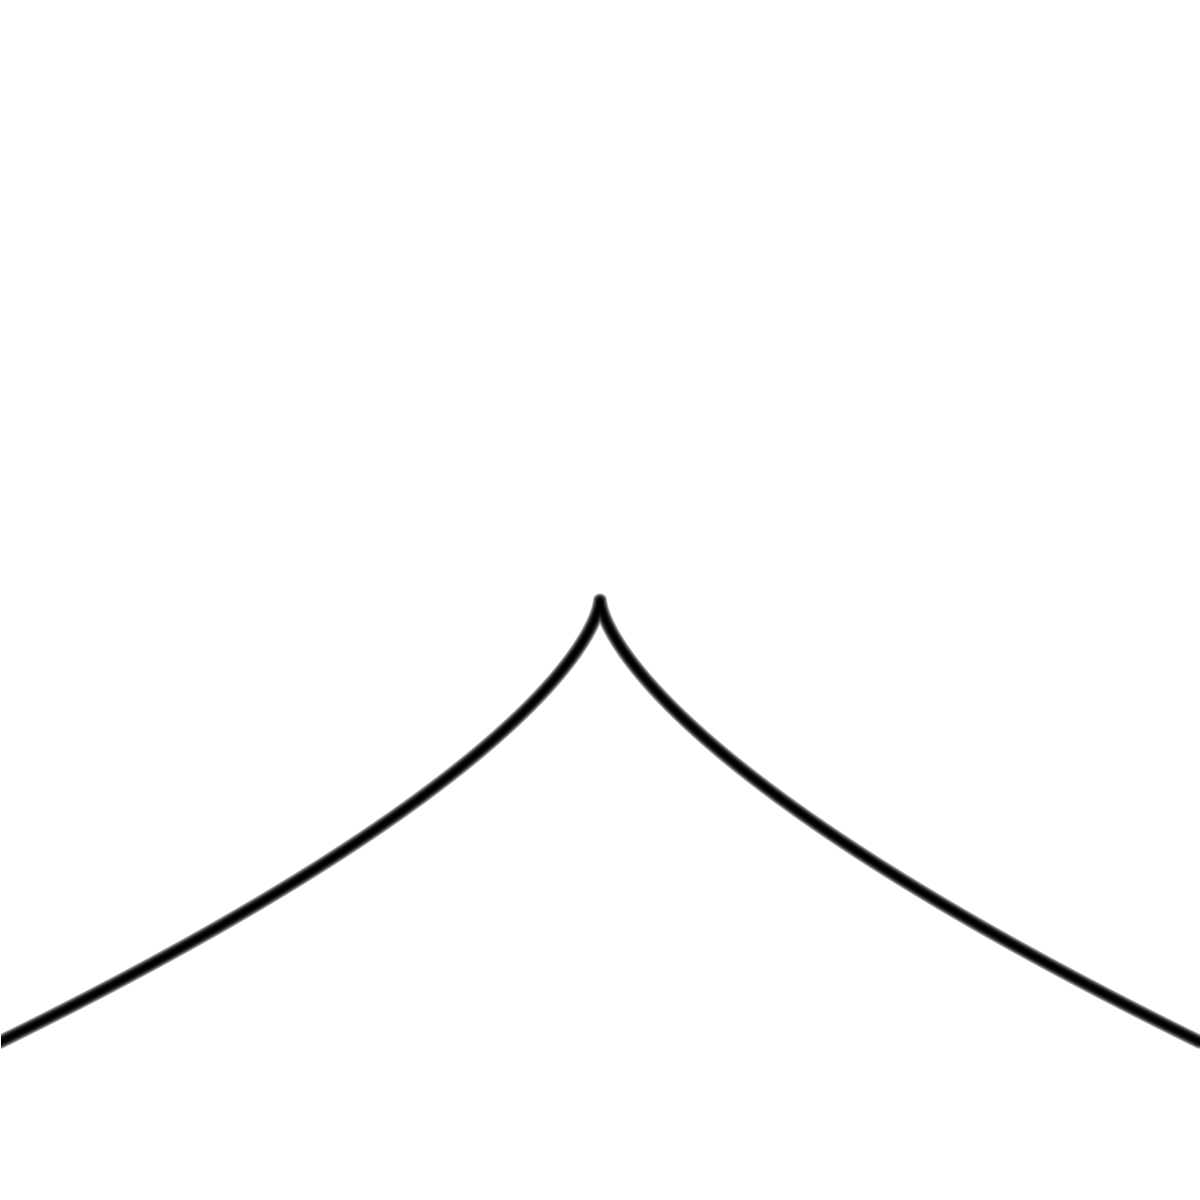
\includegraphics[width=1.2cm]{../../common/images/cuspe_def_cut_1}
        \end{tabular}
        &
        \begin{tabular}{@{}c@{}}
          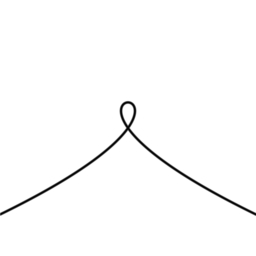
\includegraphics[width=1.2cm]{../../common/images/cuspe_def_cut_2}
        \end{tabular}
        &
        \begin{tabular}{@{}c@{}}
          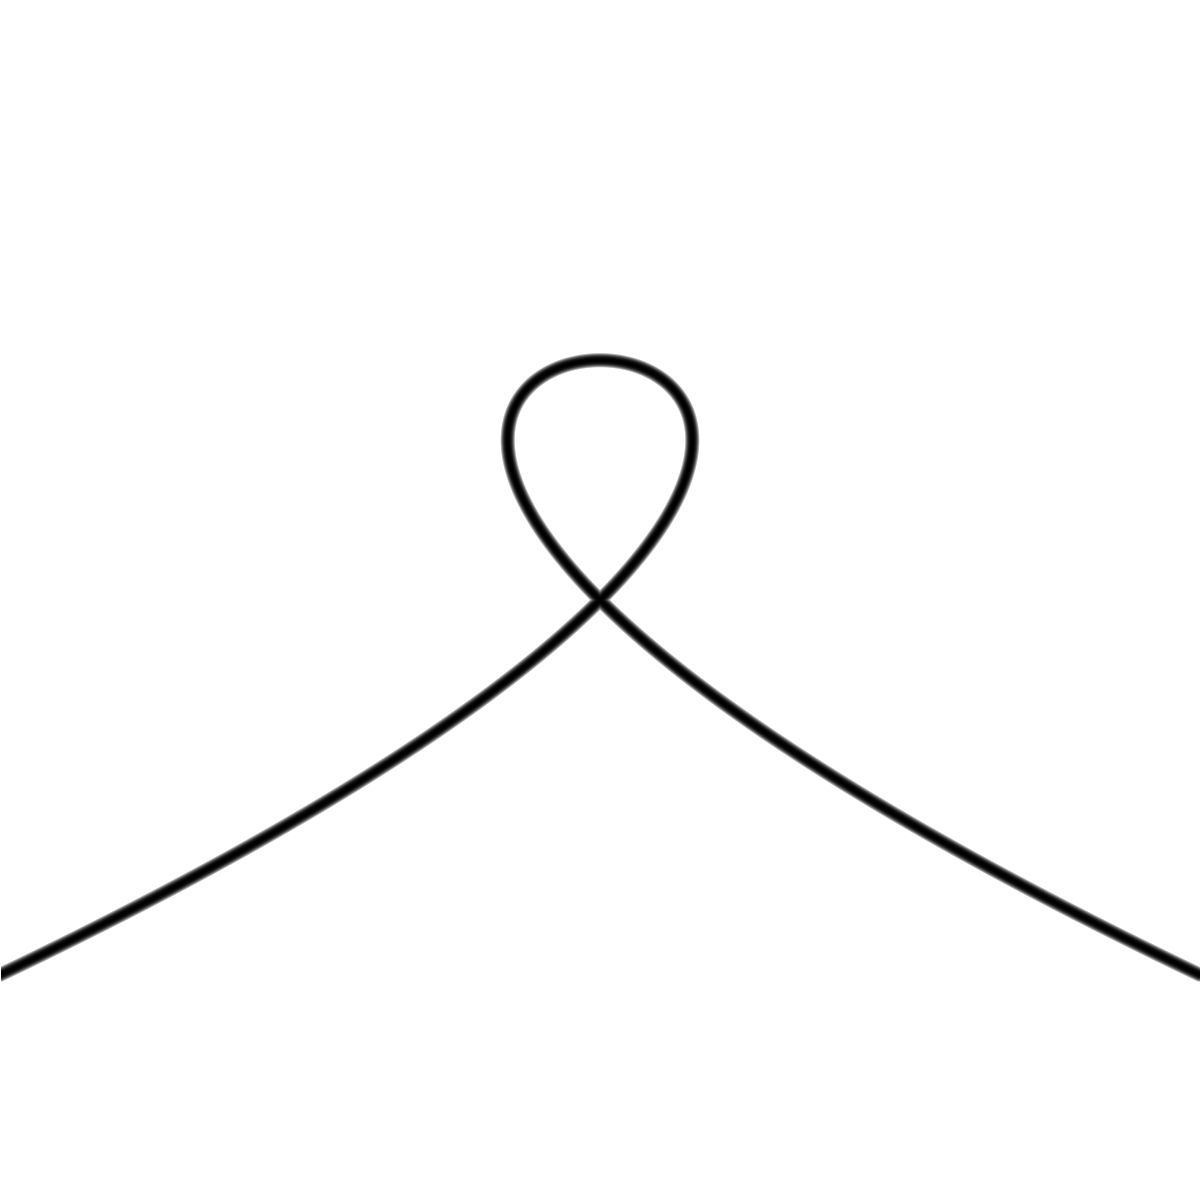
\includegraphics[width=1.2cm]{../../common/images/cuspe_def_cut_3}
        \end{tabular}
      \end{tabular}
    \end{center}
 
\end{surferPage}
